% !TeX program = pdflatex
\documentclass[12pt]{article}
\usepackage[utf8]{inputenc}
\usepackage[T1]{fontenc}
\usepackage[brazilian]{babel}
\usepackage{lmodern}
\usepackage{tgheros}
\usepackage{geometry}
\geometry{paperwidth=841mm,paperheight=1189mm,margin=0mm}
\usepackage{graphicx}
\graphicspath{{imagens/}}
\usepackage{tikz}
\usetikzlibrary{arrows.meta,calc}
\usepackage{amsmath}
\usepackage{microtype}
\usepackage[hidelinks,unicode]{hyperref}

\hypersetup{
  pdftitle={Iridologia sob Lentes Científicas: Avaliação Crítica com Aprendizado de Máquina},
  pdfauthor={Vinicius Sedrim; Vladimir Emiliano Moreira Rocha},
  pdfsubject={Iniciação Científica UFABC: avaliação crítica de imagens de íris para DM2},
  pdfkeywords={UFABC, CMCC, CNPq, iridologia, diabetes tipo 2, aprendizado de máquina},
  pdfdisplaydoctitle=true,
  pdfprintscaling=None
}

\renewcommand{\familydefault}{\sfdefault}
\pagestyle{empty}
\setlength{\parindent}{0pt}
\setlength{\parskip}{0pt}
\setlength{\emergencystretch}{1em}
\hyphenpenalty=9000
\tolerance=1400
\tracinglostchars=3

\definecolor{Ink}{HTML}{242D2B}
\definecolor{DeepForest}{HTML}{123D33}
\definecolor{Forest}{HTML}{006633}
\definecolor{Teal}{HTML}{447F75}
\definecolor{Aqua}{HTML}{DCEEE7}
\definecolor{Ice}{HTML}{F1F6F3}
\definecolor{Mist}{HTML}{D9E5E0}
\definecolor{Rule}{HTML}{CBD6D1}
\definecolor{Muted}{HTML}{52615D}
\definecolor{Gold}{HTML}{C08B22}
\definecolor{PaleGold}{HTML}{FAF1D9}
\definecolor{Coral}{HTML}{A84F43}

\newcommand{\Font}[1]{\fontsize{#1}{\dimexpr #1pt*6/5\relax}\selectfont}
\newcommand{\PosterCite}[1]{\textcolor{Teal}{\hyperlink{ref:#1}{[#1]}}}
\newcommand{\TitleSize}{68}
\newcommand{\UnitSize}{62}
\newsavebox{\PosterBlock}
\newsavebox{\PosterCapital}

\newcommand{\Block}[6]{%
  \node[anchor=north west,inner sep=0pt,outer sep=0pt,
    text=Ink,font=\normalfont\sffamily\Font{#5}] at ({#1},{#2}) {%
    \sbox{\PosterBlock}{%
      \begin{minipage}[t]{#3cm}
        \raggedright #6\par
      \end{minipage}%
    }%
    \typeout{POSTER-BLOCK (#1,#2) height=\the\dimexpr\ht\PosterBlock+\dp\PosterBlock\relax; limit=#4cm}%
    \ifdim\dimexpr\ht\PosterBlock+\dp\PosterBlock\relax>#4cm
      \PackageError{poster}{Block at (#1,#2) exceeds #4 cm}{Shorten the text or increase its reserved height.}%
    \fi
    \usebox{\PosterBlock}%
  };%
}

\newcommand{\CheckCapHeight}[2]{%
  \sbox{\PosterCapital}{{\Font{#2}\bfseries H}}%
  \typeout{POSTER-CHECK #1 capital-height=\the\ht\PosterCapital}%
  \ifdim\ht\PosterCapital<15mm
    \PackageError{poster}{#1 capital height is below 15 mm}{Increase the font size; do not scale the final PDF.}%
  \fi
}

\begin{document}
\CheckCapHeight{Title}{\TitleSize}
\CheckCapHeight{Unit}{\UnitSize}
\typeout{POSTER-CHECK paper-width=\the\paperwidth; paper-height=\the\paperheight}
\null
\begin{tikzpicture}[remember picture,overlay]
\begin{scope}[shift={(current page.north west)},x=1cm,y=-1cm]

% ----------------------------------------------------------------------
% Base and institutional header
% ----------------------------------------------------------------------
\fill[white] (0,0) rectangle (84.1,118.9);
\fill[Forest] (0,0) rectangle (84.1,0.38);
\fill[Gold] (67.0,0) rectangle (84.1,0.38);

\node[anchor=north,inner sep=0pt,outer sep=0pt] at (7.9,1.05)
  {
\includegraphics[height=5.8cm]{logo_ufabc_vertical.pdf}};
\draw[Rule,line width=1.0pt] (15.2,1.25) -- (15.2,6.9);
\Block{17.2}{1.35}{63.9}{1.2}{28}{\color{Muted}\bfseries UNIVERSIDADE FEDERAL DO ABC}
\Block{17.2}{3.15}{63.9}{3.5}{\UnitSize}{\color{Forest}\bfseries
  CENTRO DE MATEMÁTICA, COMPUTAÇÃO E COGNIÇÃO
}
\draw[Rule,line width=0.8pt] (3,7.75) -- (81.1,7.75);

% ----------------------------------------------------------------------
% Title and main finding
% ----------------------------------------------------------------------
\fill[white] (0,8.2) rectangle (84.1,21.3);
\Block{3.2}{9.4}{77.7}{5.9}{\TitleSize}{\color{Ink}\bfseries
  IRIDOLOGIA SOB LENTES CIENTÍFICAS:\\[0.15cm]
  AVALIAÇÃO CRÍTICA COM APRENDIZADO DE MÁQUINA
}
\Block{3.2}{16.65}{77.7}{1.6}{30}{\color{Forest}\bfseries
  Vinicius Sedrim\enspace\textperiodcentered\enspace Vladimir Emiliano Moreira Rocha\textsuperscript{*}
}
\Block{3.2}{18.9}{77.7}{1.3}{23}{\color{Muted}
  Bolsista CNPq\quad /\quad \textsuperscript{*}Orientador\quad /\quad Encontro de Iniciação Científica 2026
}
\fill[Ice] (0,21.3) rectangle (84.1,29.8);
\fill[Forest] (3.2,22.4) rectangle (3.45,28.65);
\Block{4.6}{23.1}{75.0}{2.2}{50}{\color{Forest}\bfseries
  Classificar não é validar clinicamente.
}
\Block{4.6}{26.1}{75.0}{1.3}{30}{
  Na avaliação realizada, o MLP alcançou \textbf{92,36\% de acurácia média}.
}

% ----------------------------------------------------------------------
% Introduction and objectives
% ----------------------------------------------------------------------
\Block{3.2}{31.5}{36.8}{1.4}{28}{\color{Forest}\bfseries 01 / INTRODUÇÃO}
\Block{44.3}{31.5}{36.6}{1.4}{28}{\color{Forest}\bfseries OBJETIVOS}
\draw[Rule,line width=0.8pt] (42.0,31.5) -- (42.0,38.4);
\Block{3.2}{33.85}{36.8}{5.0}{29}{
  A iridologia associa regiões da íris a órgãos, mas não tem validação
  diagnóstica.\,\PosterCite{1} Resultados de aprendizado de máquina para diabetes
  tipo 2 (DM2) motivam a investigação de vieses de aquisição e vazamento
  de dados.\,\PosterCite{2}\PosterCite{3}
}
\Block{44.3}{33.85}{36.6}{5.0}{29}{
  Avaliar criticamente o sinal nas imagens, comparar classificadores e testar
  sua sensibilidade ao pré-processamento. Investigar regiões locais como
  \textbf{hipóteses exploratórias}, sem presumir a validade dos mapas iridológicos.
}

% ----------------------------------------------------------------------
% Materials and methods
% ----------------------------------------------------------------------
\draw[Rule,line width=0.8pt] (3.2,39.7) -- (80.9,39.7);
\Block{3.2}{40.7}{77.7}{1.4}{28}{\color{Forest}\bfseries 02 / MATERIAIS E MÉTODOS}
\foreach \stepX/\stepTitle in {
  3.2/{1\quad IMAGEM},19.3/{2\quad SEGMENTAÇÃO},35.4/{3\quad NORMALIZAÇÃO},
  51.5/{4\quad MODELOS},67.6/{5\quad VALIDAÇÃO}} {
  \Block{\stepX}{43.0}{13.3}{1.2}{24}{\color{Forest}\bfseries \stepTitle}
}
\begin{scope}
  \clip (9.7,46.2) circle (1.65);
  \node[inner sep=0pt] at (9.7,46.2)
    {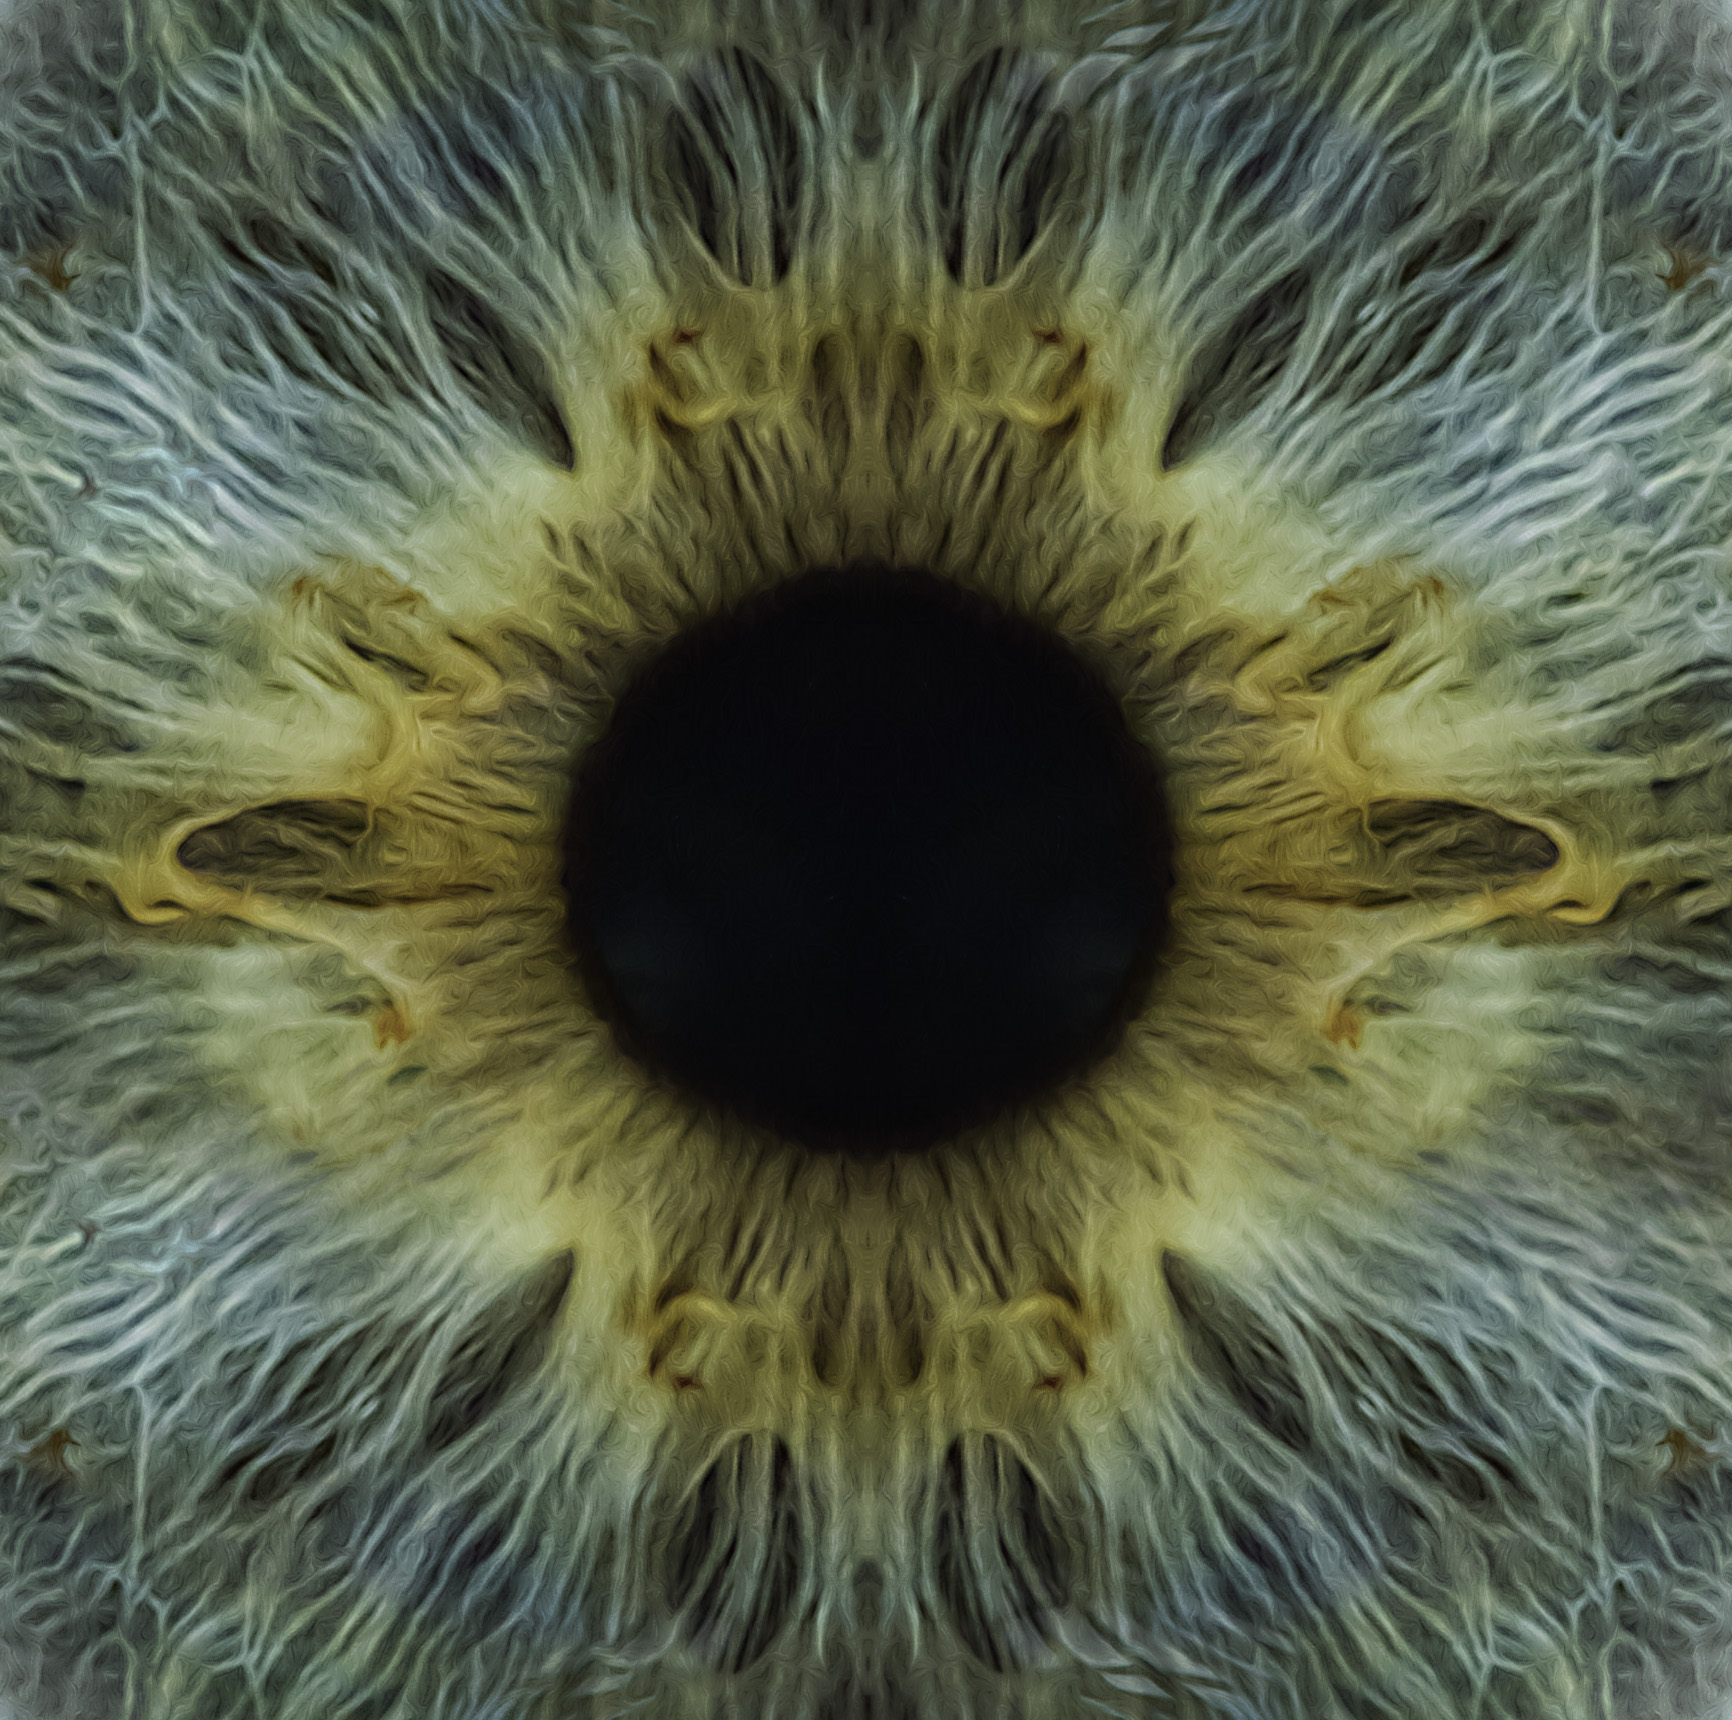
\includegraphics[width=4.3cm]{iris_closeup.jpg}};
\end{scope}
\begin{scope}[shift={(25.8,46.2)}]
  \draw[Forest,line width=1.4pt] (0,0) circle (1.65);
  \draw[Teal,line width=1.0pt] (0,0) circle (1.1);
  \fill[Ink] (0,0) circle (0.48);
  \draw[Coral,line width=1.4pt] (-1.5,0.95) .. controls (-0.7,1.4)
    and (0.8,1.3) .. (1.5,0.9);
\end{scope}
\node[inner sep=0pt] at (42.05,46.2)
  {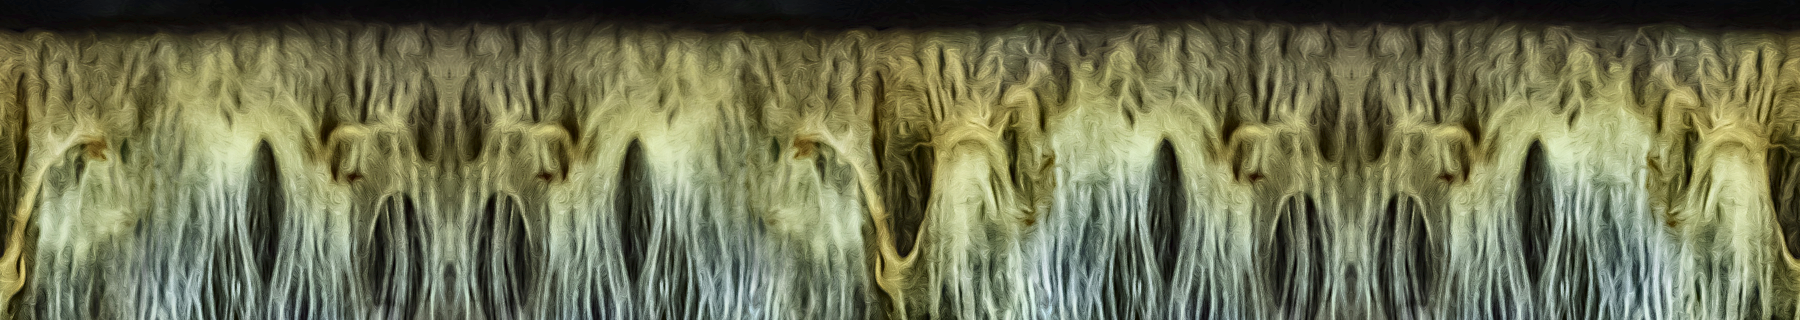
\includegraphics[width=12cm,height=3.4cm,keepaspectratio]{iris_strip_ilustrativa.png}};
\begin{scope}[shift={(54.2,44.9)}]
  \foreach \inputY in {0,1.3,2.6} {
    \foreach \hiddenY in {0.4,2.2} {
      \draw[Teal!60,line width=0.9pt] (0,\inputY) -- (3.4,\hiddenY);
      \draw[Teal!60,line width=0.9pt] (3.4,\hiddenY) -- (6.8,\inputY);
    }
    \fill[Forest] (0,\inputY) circle (0.17);
    \fill[Forest] (6.8,\inputY) circle (0.17);
  }
  \fill[Gold] (3.4,0.4) circle (0.21);
  \fill[Gold] (3.4,2.2) circle (0.21);
\end{scope}
\foreach \fold in {0,...,4} {
  \foreach \group in {0,...,4} {
    \ifnum\fold=\group
      \fill[Gold] ({69.0+\group*1.9},{44.65+\fold*0.61})
        rectangle ({70.6+\group*1.9},{45.1+\fold*0.61});
    \else
      \fill[Mist] ({69.0+\group*1.9},{44.65+\fold*0.61})
        rectangle ({70.6+\group*1.9},{45.1+\fold*0.61});
    \fi
  }
}
\foreach \arrowX in {17.1,33.2,49.3,65.4} {
  \draw[Muted,line width=1.2pt,-{Stealth[length=3.5mm,width=2.5mm]}]
    (\arrowX,46.2) -- ({\arrowX+1.2},46.2);
}
\Block{3.2}{48.8}{13.3}{2.5}{25}{Íris e rótulos de diabetes ou controle.}
\Block{19.3}{48.8}{13.3}{2.5}{25}{Delimitar íris e pupila; reduzir artefatos.}
\Block{35.4}{48.8}{13.3}{2.5}{25}{Mapeamento polar; intensidades dos pixels.}
\Block{51.5}{48.8}{13.3}{2.5}{25}{LR, SVM, RF, MLP e AdaBoost.}
\Block{67.6}{48.8}{13.3}{2.5}{25}{5 \textit{folds}; isolamento por pessoa a verificar.}
\Block{3.2}{52.0}{77.7}{0.9}{18}{\color{Muted}
  Fluxo metodológico; imagens ilustrativas. Foto: Carlos Andrés Reyes / Wikimedia Commons, CC BY 2.0.
  Faixa polar: adaptação da foto.
}
\Block{3.2}{53.5}{77.7}{1.2}{25}{
  \textbf{Protocolo reportado:} 5 \textit{folds}, semente 42 e padronização calculada apenas no treino.
}

% ----------------------------------------------------------------------
% Results and discussion
% ----------------------------------------------------------------------
\fill[Ice] (0,55.7) rectangle (84.1,59.3);
\Block{3.2}{56.25}{77.7}{1.4}{30}{\color{Forest}\bfseries 03 / RESULTADOS E DISCUSSÃO}
\Block{3.2}{58.0}{77.7}{1.0}{23}{\color{Ink}
  Resultados preliminares da avaliação interna, sujeitos à reanálise após a auditoria da base.
}
\Block{3.2}{60.4}{46.0}{1.5}{29}{\bfseries Comparação global dos cinco modelos}
\foreach \tick in {80,85,90,95,100} {
  \pgfmathsetmacro{\tickX}{12.5+(\tick-80)*1.525}
  \draw[Rule,line width=0.7pt] (\tickX,62.1) -- (\tickX,74.5);
  \node[anchor=north,font=\Font{22},text=Muted,inner sep=0pt]
    at (\tickX,75.0) {\tick};
}
\foreach \model/\mean/\deviation/\rowY/\modelColor/\valueLabel in {
  MLP/92.36/3.59/63.2/Forest/{92,36},
  LR/90.81/3.50/65.7/Teal/{90,81},
  SVM/88.24/6.22/68.2/Teal/{88,24},
  AdaBoost/87.79/5.07/70.7/Teal/{87,79}} {
  \pgfmathsetmacro{\meanX}{12.5+(\mean-80)*1.525}
  \pgfmathsetmacro{\lowX}{12.5+(\mean-\deviation-80)*1.525}
  \pgfmathsetmacro{\highX}{12.5+(\mean+\deviation-80)*1.525}
  \node[anchor=west,font=\Font{28}\bfseries,text=Ink,inner sep=0pt]
    at (3.2,\rowY) {\model};
  \draw[\modelColor,line width=2.4pt] (\lowX,\rowY) -- (\highX,\rowY);
  \draw[\modelColor,line width=1.6pt] (\lowX,{\rowY-0.28}) -- (\lowX,{\rowY+0.28});
  \draw[\modelColor,line width=1.6pt] (\highX,{\rowY-0.28}) -- (\highX,{\rowY+0.28});
  \fill[\modelColor] (\meanX,\rowY) circle (0.21);
  \node[anchor=east,font=\Font{28}\bfseries,text=\modelColor,inner sep=0pt]
    at (49.2,\rowY) {\valueLabel\%};
}
\node[anchor=west,font=\Font{28}\bfseries,text=Ink,inner sep=0pt] at (3.2,73.2) {RF\textsuperscript{*}};
\draw[Muted,line width=1.6pt,fill=white] ({12.5+(83.67-80)*1.525},73.2) circle (0.21);
\node[anchor=east,font=\Font{28}\bfseries,text=Muted,inner sep=0pt] at (49.2,73.2) {83,67\%};
\Block{3.2}{76.6}{46.0}{2.2}{22}{\color{Muted}
  Acurácia (\%). Pontos: médias; hastes: $\pm$1 DP entre 5 \textit{folds}, não intervalos de confiança.
  \textsuperscript{*}RF: DP não reportado. Não se estabelece superioridade estatística.
}

\draw[Rule,line width=0.8pt] (52.0,60.4) -- (52.0,78.5);
\Block{54.2}{60.4}{26.7}{1.4}{28}{\color{Coral}\bfseries AUDITORIA DOS DADOS}
\Block{54.2}{62.6}{26.7}{1.3}{23}{\color{Muted}Auditoria posterior da base legada}
\Block{54.2}{65.0}{10.2}{2.0}{48}{\bfseries 196}
\Block{70.0}{65.0}{10.9}{2.0}{48}{\color{Forest}\bfseries 123}
\draw[Muted,line width=1.3pt,-{Stealth[length=4mm,width=3mm]}] (65.0,66.0) -- (68.5,66.0);
\Block{54.2}{67.35}{10.2}{1.0}{23}{entradas}
\Block{70.0}{67.35}{10.9}{1.5}{23}{imagens únicas}
\Block{54.2}{69.5}{26.7}{1.4}{27}{\bfseries 73 cópias exatas removidas.}
\Block{54.2}{71.8}{26.7}{3.5}{28}{
  Sem IDs pessoais e sem confirmação do subtipo DM2.
  \textbf{O nome da partição não comprova isolamento por pessoa.}
}
\Block{54.2}{75.5}{26.7}{3.1}{22}{\color{Muted}
  As contagens auditadas não comprovam o tamanho amostral da avaliação preliminar.
  Base vinculada ao \textbf{artigo retratado de Moradi et al.}\,\PosterCite{4}
}
\fill[Ice] (3.2,79.4) rectangle (80.9,81.0);
\Block{4.0}{79.75}{76.1}{1.0}{23}{
  \textbf{MLP, métricas reportadas:}\quad sensibilidade 92,60\%\quad especificidade 92,10\%\quad F1 92,70\%.
}

\Block{3.2}{82.5}{38.5}{1.6}{30}{\bfseries Robustez fotométrica}
\Block{3.2}{84.6}{38.5}{1.6}{23}{\color{Muted}
  MLP: diferença em relação ao original (pp).
  Mesma representação-base de pixels.
}
\node[anchor=east,font=\Font{19},text=Muted,inner sep=0pt] at (41.7,86.6) {Acurácia};
\foreach \tick/\tickLabel in {-0.6/{-0,6},-0.4/{-0,4},-0.2/{-0,2},0/{0}} {
  \pgfmathsetmacro{\tickX}{37.5+\tick*23.5}
  \draw[Rule,line width=0.7pt] (\tickX,87.5) -- (\tickX,96.2);
  \node[anchor=north,font=\Font{20},text=Muted,inner sep=0pt] at (\tickX,96.7) {\tickLabel};
}
\foreach \transform/\value/\rowY/\pointColor/\valueLabel in {
  Original/92.36/87.8/Forest/{92,36},
  Equalização global/92.33/89.7/Teal/{92,33},
  CLAHE/92.18/91.6/Teal/{92,18},
  Desfoque gaussiano/91.74/93.5/Coral/{91,74},
  Composição/91.96/95.4/Teal/{91,96}} {
  \pgfmathsetmacro{\pointX}{37.5+(\value-92.36)*23.5}
  \node[anchor=west,font=\Font{24},text=Ink,inner sep=0pt] at (3.2,\rowY) {\transform};
  \draw[\pointColor,line width=1.8pt] (\pointX,\rowY) -- (37.5,\rowY);
  \fill[\pointColor] (\pointX,\rowY) circle (0.16);
  \node[anchor=east,font=\Font{22}\bfseries,text=\pointColor,inner sep=0pt]
    at (41.7,\rowY) {\valueLabel\%};
}
\Block{3.2}{98.25}{13.3}{2.0}{40}{\color{Coral}\bfseries 0,62 pp}
\Block{17.5}{98.3}{24.2}{2.4}{25}{Maior queda reportada, sob desfoque gaussiano.}
\Block{3.2}{101.15}{38.5}{2.8}{22}{\color{Muted}
  Composição: equalização global + CLAHE + desfoque.
  CLAHE: equalização adaptativa com limite de contraste.
  Não testa generalização para novas câmeras ou populações.
}

\draw[Rule,line width=0.8pt] (43.5,82.5) -- (43.5,104.0);
\Block{45.3}{82.5}{35.6}{1.6}{30}{\bfseries Análise local exploratória}
\Block{45.3}{84.6}{35.6}{1.5}{23}{\color{Muted}LR + equalização global; grade da região de interesse.}
\foreach \row [count=\rowIndex from 0] in {
  {61,62,60,58,59,61,63,60,58,59,60,61},
  {62,65,68,64,62,65,67,62,60,61,62,63},
  {60,68,88,91,89,70,65,61,59,60,61,60},
  {59,66,92,95,90,72,64,60,58,59,60,62},
  {61,64,87,89,86,69,63,62,60,61,63,61},
  {63,62,65,67,64,62,61,64,62,63,61,60},
  {60,61,63,65,62,60,59,61,63,60,59,58},
  {58,60,61,62,60,59,58,60,61,62,60,59},
  {59,59,60,61,59,58,57,59,60,61,59,58},
  {60,61,62,60,58,59,60,62,63,60,58,59},
  {61,62,61,59,60,61,62,61,62,61,60,60},
  {58,60,59,58,59,60,61,59,58,59,60,61}} {
  \foreach \accuracy [count=\columnIndex from 0] in \row {
    \pgfmathsetmacro{\cellShade}{100*(\accuracy-55)/40}
    \pgfmathsetmacro{\cellX}{46.0+1.06*\columnIndex}
    \pgfmathsetmacro{\cellY}{87.0+1.06*\rowIndex}
    \fill[Forest!\cellShade!Mist]
      (\cellX,\cellY) rectangle ({\cellX+1.015},{\cellY+1.015});
  }
}
\foreach \index in {0,3,6,9,11} {
  \node[anchor=south,font=\Font{18},text=Muted,inner sep=0pt]
    at ({46.53+1.06*\index},86.7) {\index};
  \node[anchor=east,font=\Font{18},text=Muted,inner sep=0pt]
    at (45.65,{87.53+1.06*\index}) {\index};
}
\draw[Gold,line width=2.0pt] (49.18,90.18) rectangle (50.195,91.195);
\foreach \band in {0,...,39} {
  \pgfmathsetmacro{\shade}{100*(39-\band)/39}
  \fill[Forest!\shade!Mist] (60.1,{87.0+\band*0.318})
    rectangle (61.0,{87.0+(\band+1)*0.318});
}
\foreach \legendY/\legendLabel in {87.0/{95\%},93.36/{75\%},99.72/{55\%}} {
  \node[anchor=west,font=\Font{20},text=Muted,inner sep=0pt]
    at (61.5,\legendY) {\legendLabel};
}
\Block{67.0}{87.7}{13.9}{2.1}{52}{\color{Forest}\bfseries 95\%}
\Block{67.0}{90.4}{13.9}{2.3}{26}{pico reportado na célula (3,3).}
\Block{67.0}{93.6}{13.9}{2.6}{25}{144 células avaliadas; seleção exploratória.}
\Block{67.0}{97.1}{13.9}{2.3}{25}{\bfseries Não é a acurácia global.}
\Block{45.3}{101.15}{35.6}{2.8}{24}{\color{Muted}
  Sem correção para múltiplas comparações.
  A localização exige confirmação independente, não valida uma associação entre íris e pâncreas.
}

% ----------------------------------------------------------------------
% Conclusions and next steps
% ----------------------------------------------------------------------
\fill[DeepForest] (0,105.2) rectangle (84.1,112.0);
\Block{3.2}{106.3}{77.7}{1.2}{26}{\color{Aqua}\bfseries 04 / CONCLUSÕES}
\Block{3.2}{108.1}{77.7}{1.6}{34}{\color{white}\bfseries
  Acurácia alta não substitui dados rastreáveis nem validação externa.
}
\Block{3.2}{110.2}{77.7}{1.8}{27}{\color{white}
  Próximos passos: confirmar proveniência, licença, IDs e rótulos clínicos;
  recalcular com múltiplas sementes e validar em uma coorte independente.
}

% ----------------------------------------------------------------------
% Footer: acknowledgments, references, and image credits
% ----------------------------------------------------------------------
\Block{3.2}{112.9}{18.8}{0.9}{20}{\color{Forest}\bfseries AGRADECIMENTOS}
\Block{3.2}{114.3}{18.8}{3.5}{19}{
  Este trabalho foi financiado pelo CNPq, no âmbito da Iniciação Científica da UFABC.
  Agradeço ao orientador pelo apoio.
}
\Block{24.2}{112.9}{36.4}{0.9}{20}{\color{Forest}\bfseries REFERÊNCIAS BIBLIOGRÁFICAS}
\Block{24.2}{114.3}{36.4}{4.0}{16}{
  \hypertarget{ref:1}{\textbf{[1]}} ERNST, E. Iridology: a systematic review.
  \textit{Arch. Ophthalmol.}, 118:120--121, 2000.\par
  \hypertarget{ref:2}{\textbf{[2]}} SAMANT, P.; AGARWAL, R. Machine learning techniques for medical
  diagnosis of diabetes using iris images. \textit{CMPB}, 157:121--128, 2018.\par
  \hypertarget{ref:3}{\textbf{[3]}} ZECH, J. R. et al. Variable generalization performance of a deep
  learning model to detect pneumonia in chest radiographs: a cross-sectional study.
  \textit{PLOS Med.}, 15:e1002683, 2018.\par
  \hypertarget{ref:4}{\textbf{[4]}} MORADI, P. et al. Retraction Notice: Discovering Informative
  Regions in Iris Images to Predict Diabetes. \textit{ICBME}.
  \href{https://doi.org/10.1109/ICBME45317.2018.10207763}{doi:10.1109/ICBME45317.2018.10207763}.
}
\Block{63.0}{112.9}{17.9}{0.9}{20}{\color{Forest}\bfseries IMAGENS E FONTES}
\Block{63.0}{114.3}{17.9}{3.5}{16}{
  Foto: Carlos Andrés Reyes,
  \href{https://commons.wikimedia.org/wiki/File:Iris_eclipse_-_Explored_-_Flickr_-_creyesk.jpg}{\textit{Iris eclipse}}, Wikimedia Commons.
  \href{https://creativecommons.org/licenses/by/2.0/}{CC BY 2.0}.
  Faixa polar: adaptação ilustrativa (remapeamento e contraste).
  Logo: UFABC / Sucom. Gráficos e esquemas: autoria própria.
}

\end{scope}
\end{tikzpicture}
\end{document}
